
\chapter{Algorithms for Partial Coloring}
\label{ch:partial-alg}
In Chapter \ref{ch:partial}, we saw the partial coloring method, and how it can give substantially improved bounds for various problems.
For a long time however, no efficient algorithms were known for these methods, which prevented the use of discrepancy in many algorithmic applications. Interestingly, in recent years, several algorithmic approaches have been developed for these, based on ideas from probability, linear algebra, geometry and optimization.

In this chapter, we describe two such elegant results. First, the Edge-Walk algorithm due to Lovett and Meka, that gives an algorithmic version of Theorem \ref{lm:ch3-partial}. Second, an algorithm due to Rothvoss for the more general setting of arbitrary symmetric convex bodies in Theorem \ref{lm:ch3-gian}.
In Section \ref{sec:vec-herdisc}, we describe the notion of vector discrepancy and an algorithm for finding low discrepancy colorings based on semidefinite programming.





\section{Lovett-Meka Algorithm}
\label{sec:lm}
Recall the setting of Theorem \ref{lm:ch3-partial}, where we are given $m$ vectors $v_1, \ldots, v_m \in \R^n$, and real parameters $\lambda_1,\ldots, \lambda_m\geq 0$, and the goal is to find a partial coloring $x$ such that $ |\ip{v_i,x}| \leq \lambda_i \|v_i\|_2 $. 

We will show the following result.
%the algorithm was also truly constructive as it did not rely on Theorem \ref{th:pcol} to argue feasibility.

%As usual, let $(V,C)$ be a set system with $n$ elements and $m$ sets $S_1,\ldots,S_m$.
%Lovett and Meka  \cite{LM12} gave the following algorithmic version of the partial coloring lemma.

\begin{theorem}
\label{th:lm}
Let $v_1, \ldots, v_m \in \R^n$,  and let $x_0 \in [-1,1]^n$ be some arbitrary starting point, and let   $\lambda_1,\ldots,\lambda_m \geq 0$ be such that 
\begin{equation}
\label{eqcond21}
 \sum_i \exp(-\lambda_i^2/16) \leq n/16.
 \end{equation}
 Let $\delta>0$ be an arbitrarily small parameter.
Then there is a randomized algorithm that runs in time polynomial in $n,m$ and $1/\delta$, and,  with constant probability, finds $x\in [-1,1]^n$ such that
\smallskip 

(i) $|\{i: |x(i)| \geq 1-\delta\}| \ge \frac{n}{2}$, and 

\smallskip

(ii)  $|\ip{v_i,x-x_0}| \leq \lambda_i \|v_i\|_2$ for each $i\in [m]$.
\end{theorem}

\begin{remark} We set $\delta = 1/\text{poly}(n,m)$ to keep the running time polynomial, 
 but it is convenient to think of $\delta$ as $0$. So (i) says that the colors of at least $n/2$ elements reach $\pm 1$, and (ii) controls the discrepancy incurred for each vector.
 
The ``colors'' $x(i)$ produced by the algorithm in Theorem \ref{th:lm} lie in $[-1,1]$, in contrast to $\{-1,0,1\}$ in Theorem \ref{lm:ch3-partial}. 
But this makes no difference in applications as the starting point $x_0$ is allowed to be arbitrary, and we can iterate the algorithm for $O(\log n)$ rounds to obtain a full coloring.
In fact, this flexibility in colors allows the condition in \eqref{eqcond21} to be more relaxed than in \eqref{eq:ch3-partial}. In particular, the contribution of any $\lambda_i$ to the left side in \eqref{eqcond21} never exceeds $1$, while $\parcol(\lambda_i)$ in \eqref{eq:ch3-partial} gets arbitrarily large as $\lambda_i$ approaches $0$.
\end{remark}


%The  reader may assume that the starting coloring $x$ is $(0,\ldots,0)$.

%$\lambda=0$ for $\Omega(n)$ sets. 
%For more discussion on the comparison with the entropy method we refer the reader to \cite{LM12}.


%Moreover, it suffices to do a standard Brownian motion in this subspace and no SDP is needed.
%Besides 

% We now prove theorem \ref{th:lm}.
% Let $K$ denote the set of alive elements at $t=0$.
% Without loss of generality let us assume that $K=\{1,\ldots,k\}$.
% As in the previous algorithms, the algorithm will start from the initial coloring $x_0=x$ and update it over time as $x_t = x_{t-1} + u^t$  by adding a suitably chosen tiny update vector $u^t$ at time $t$.

\subsection{The Algorithm}
At a high level, the algorithm is based on combining the linear algebraic approach from  Chapter \ref{ch:linalg} with probabilistic techniques.
%We first give an informal description.
% The key idea of the algorithm is that whenever a discrepancy constraint becomes tight or some variable reaches $\pm 1$, one can simply do a random walk orthogonal to it. We now describe it formally. Wlog we assume that all variables are initially alive, i.e.,~$k=n$.
%Without loss of generality, let us assume that $k=n$.

\medskip
\noindent {\bf The idea.}
The algorithm starts at the point $x_0$, and performs a standard Brownian motion (approximated by a random walk with tiny Gaussian increments). See Figure \ref{fig:lm} below. Let $x_t$ denote the coloring at time $t$. If some coordinate $x_t(j)$ reaches $\pm 1$, its value is fixed and no longer updated (i.e.,~all subsequent steps of the walk are orthogonal to $e_j$, the $j$-th standard basis vector).
Moreover, if any discrepancy constraint becomes tight, i.e.,~$|\ip{v_i, x_t-x_0}| = \lambda_i \|v_i\|_2$, all the subsequent steps of the walk are orthogonal to $v_i$. 

Clearly, by design, the coloring $x_t$ stays inside the cube $[-1,1]^n$, and no discrepancy constraint  is violated.  
Notice that every time some coordinate reaches $\pm 1$, or a discrepancy constraint becomes tight, the dimension of the subspace where the walk is performed may reduce by $1$.
The key idea of the analysis is to show that the condition \eqref{eqcond21} ensures that many coordinates are likely to reach $\pm 1$, before the walk gets ``stuck''. 
To see why this might be the case, consider the case when all $\lambda_i$ are equal, and, therefore, equal to a large enough constant $C$. Suppose also for simplicity, that $x_0 = 0$. Then the boundary of the strip $\{x: |\ip{v_i, x}| \le C \|v_i\|_2\}$, which encodes a discrepancy constraint, is at Euclidean distance $C$ from the origin, while the boundary of the cube $[-1,1]^n$ is at distance $1$ from the origin. So, intuitively, the Brownian motion is more likely to hit the boundary of the cube before a discrepancy constraint becomes tight. 



\begin{figure}[hbtp!]
    \centering
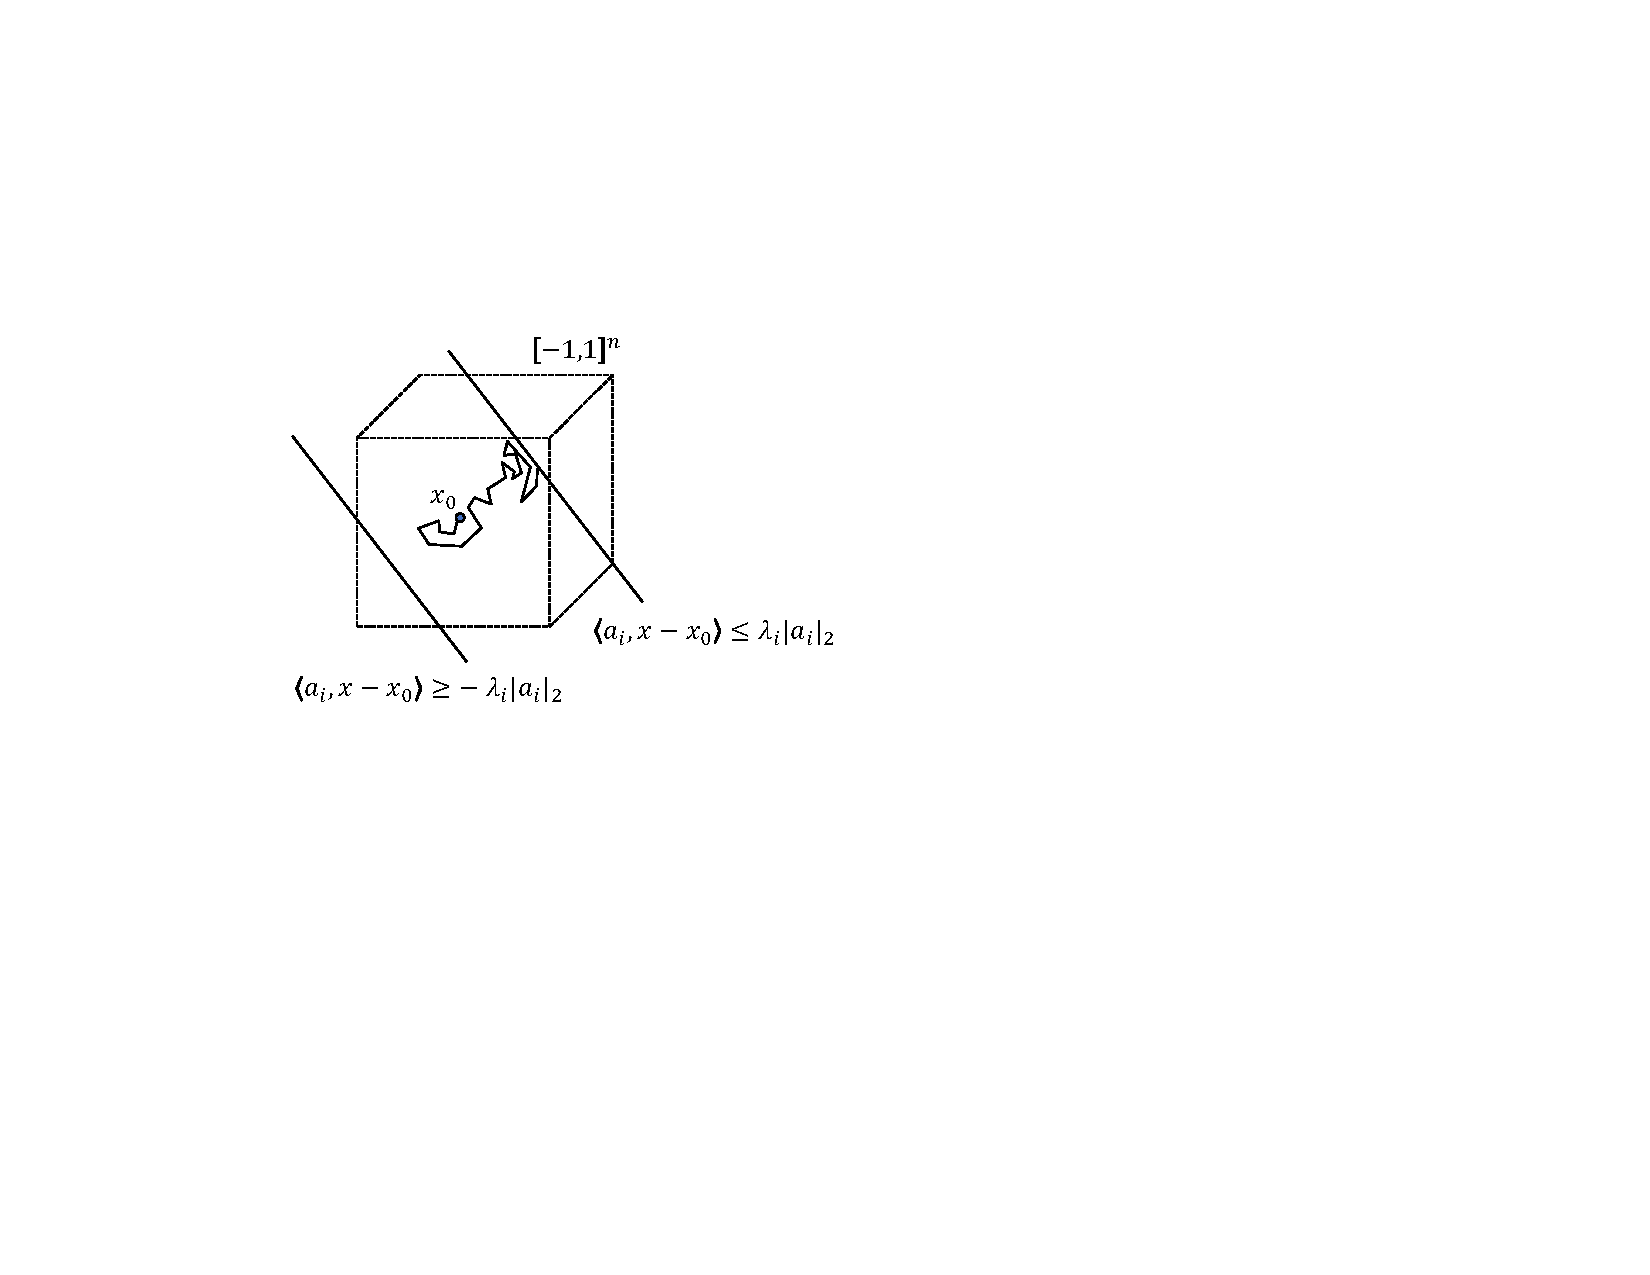
\includegraphics[scale=0.7]{ch4-figures/figures-lm.pdf}
    \caption{Lovett-Meka Algorithm. The random walk starting from $x_0$, and hitting a discrepancy constraint.}
    \label{fig:lm}
\end{figure}
\paragraph{The Formal Algorithm.}
Fix a small step size $\gamma > 0$, such that $\delta \ge c \gamma \log^{1/2}(2nm/\gamma)$ for a sufficiently large constant $c$, to be determined later. 
%Also, without loss of generality, we can assume that initially $|x_0(j)|< 1-\delta$ for each $j \in [n]$.
The algorithm proceeds in discrete time steps $t=1,2,\ldots,\ell=4/\gamma^2$.
Let $x_{t-1}$ denote the coloring at the beginning of time step $t$ (equivalently, at the end of time step  $t-1$). 
At each $t=1,\ldots,\ell$, the coloring $x_{t-1}$ is updated to $x_t$ as follows:

\smallskip

(i) Let 
$F_{t}:=\{j \in [n]: |x_{t-1}(j)|> 1-\delta \}$
denote the set of tight (\ie, \emph{fixed}) elements thus far, and let \[D_t := \{i \in [m]: |\ip{v_i,x_{t-1}-x_0}| \geq  (\lambda_i -\delta)\|v_i\|_2 \}\] denote the set of tight discrepancy constraints thus far (\ie, the \emph{dangerous} directions).

\smallskip

(ii) Let $W_t := \{ u \in \R^n: u(j)=0 \text{ for all } j \in F_t,\, \ip{v_i,u}=0 \text{ for all } i \in D_t\}$
be the subspace orthogonal to the tight constraints.
% The algorithm maintains a linear subspace $V_{t-1} \subset \R^n$.  Initially at $t=1$, the coloring is $x_0$, $A_0=[n]$ and $V_0 = \R^n$. The following is repeated for $\ell = O(\gamma^{-2})$ steps.

\smallskip 
(iii) 
Sample a random standard Gaussian vector  $g_t \sim N(W_t)$  in the subspace $W_t$, and set  $x_t = x_{t-1} + \gamma g_t$.

Above, for a linear subspace $W$ of $\R^n$, we use the notation $N(W)$ to denote the standard Gaussian distribution restricted to $W$, and $g \sim N(V)$ to mean that $g$ is a random variable distributed according to $N(V)$. 

%I.e., $g \in V$ with probability $1$, and, for any measurable $S \subseteq V$, 
%\[
%\Pr[g \in S] 
%= \frac{1}{(2\pi)^{\dim(V)/2}} \int_{S}e^{-%
%\]

\subsection{Analysis}
We show that the algorithm satisfies the guarantee in Theorem \ref{th:lm}. 

Notice that at any time $t$, we have that $x_t-x_0 = \sum_{s=1}^t \gamma g_{s}$, where each $g_s \sim N(W_s)$. As the subspace $W_s$ depends on $x_{s-1}$, which in turn depends on $g_1,\ldots,g_{s-1}$, the coloring $x_t$ evolves as a martingale with Gaussian increments.

So let us begin by recalling some basic properties of Gaussians and martingales. The analysis is elementary, and follows directly from these properties. 



\medskip 
\noindent {\bf Some properties of Gaussians.} Let us use the notation $N(\mu,\sigma^2)$ for the one-dimensional Gaussian distribution with mean $\mu$ and variance $\sigma^2$, and $g\sim N(\mu,\sigma^2)$ to denote that $g$ is a random variable distributed according to $N(\mu,\sigma^2)$. If $g_1 \sim N(\mu_1,\sigma_1^2)$  and $g_2 \sim N(\mu_2,\sigma_2^2)$ are independent Gaussians, their sum is also Gaussian with $g_1 + g_2 \sim N(\mu_1 + \mu_2, \sigma_1^2 + \sigma_2^2)$ . 
This implies that if $g = (g(1),\ldots,g(n))$ is the standard gaussian random vector in $\R^n$, with $g(1),\ldots,g(n)$ independent samples from $ N(0,1)$, then for any $u \in \R^n$, we have  \[\ip{g,u}  = \sum_i g(i) u(i) \sim N(0,\|u\|_2^2).\]
%As the algorithm proceeds, the subspaces satisfy $V_0 \supseteq V_1 \supseteq \cdots \supseteq V_\ell$. 
%Moreover, as
%  the update $\gamma g$ lies in  $V^t$, it follows that for any element $i$, we have that $|x_t(i)|$ is at most $1 - \delta + O(\sqrt{\log (T)}) \gamma  \leq 1$  with high probability. Similarly, the additional discrepancy
%  $|x_{t-1}(S) - x_0(S)|$ of any set does not exceed $\lambda_j - \delta + O(\gamma \sqrt{|S_j|} \sqrt{\log T}) \leq \lambda_j + 1/n$.
For a linear subspace $W$, and $N(W)$, as above, the standard Gaussian distribution restricted to $W$, rotational invariance implies that a random vector $g \sim N(W)$ can be written as 
$g=  g(1) w_1+ \cdots + g(d) w_d$ for any orthonormal basis
$\{w_1,\ldots,w_d\}$ for $W$ and $g(1),\ldots,g(d)$ independent samples from $N(0,1)$. %By the rotational invariance of the multi-dimensional gaussian distribution, it is easily seen that
%$g$ is invariant of the choice of the basis $\{v_1,\ldots, v_d\}$.
This implies the following useful facts.
\begin{lemma}
\label{lem:gaussian-subspace}
Let $W$ be a subspace of $\mathbb{R}^n$ of dimension $d$ and $g\sim N(W)$. Then for all $u \in \mathbb{R}^n$,  $\langle g,u \rangle \sim N(0,\sigma^2)$ with $\sigma^2 \leq \|u\|_2^2$. Moreover, $\sum_{i=1}^n \E[g(i)^2] = d$.
%Moreover, let $e_1,\ldots,e_n$ denote the standard basis vectors of $\R^n$, and let $\sigma_i$ be such that $\langle g,e_i\rangle \sim N(0,\sigma_i^2)$. Then $\sum_{i=1}^n \sigma_i^2 = d$.
\end{lemma}
\begin{proof}
Let $P$ be the orthogonal projection onto $W$.
 As $g\in W$, for any $u \in \R^n$, $\langle g,u \rangle  =  \langle g,Pu\rangle$ and  hence $\ip{g,u} \sim N(0,\|Pu\|^2)$. Clearly, $\|Pu\|_2 \leq \|u\|_2$. 
 
 For the second part, if $w_1,\ldots,w_d$ is an orthonormal basis for $W$, and $e_1, \ldots, e_n$ is the standard basis of $\R^n$, then by the above observation, 
 \[
 \E[g(i)^2] = \E[\ip{g, e_i}^2] = \|Pe_i\|_2^2 =\sum_{j=1}^d \ip{e_i,w_j}^2.
 \]
 We thus have
 \begin{align*}
     \sum_{i=1}^n \E[g(i)^2]
     = \sum_{i=1}^n \sum_{j=1}^d \ip{e_i,w_j}^2
     = \sum_{j=1}^d \sum_{i=1}^n \ip{e_i,w_j}^2
     = \sum_{j=1}^d \|w_j\|_2^2 = d,
 \end{align*}
 where the third equality follows as $\{e_1,\ldots,e_n\}$ is an orthonormal basis for $\mathbb{R}^n$.
 \end{proof}
Finally, we need some concentration properties for martingales with Gaussian increments.
Recall that for  $g \sim N(0,1)$, for any $\lambda \geq  0$, \[\Pr[ |g| \geq \lambda] \leq 2\exp(-\lambda^2/2).\]
(In fact, the factor $2$ is not necessary.) More generally, we have the following.
\begin{lemma}
\label{ch4:lm-martingale-bound}
Let $g_1,\ldots,g_\ell$ be random variables over $\R$ such that, for all $1 \leq t \leq \ell$,  $g_t$ only depends on $g_1,\ldots,g_{t-1}$, and the law of $g_t$ conditioned on $g_1, \ldots g_{t-1}$ is, with probability $1$, equal to that of a Gaussian with mean zero and variance at most $\sigma^2$.
  Then for any $\lambda > 0$, \[\Pr[|g_1 + \cdots + g_\ell| \geq  \lambda  \sqrt{\ell}\sigma] \leq  2\exp(-\lambda^2/2).\]
\end{lemma}
\begin{proof}
Recall that for $g \sim N(0,\sigma^2)$, its moment generating function is $\E[ \exp(\beta g)] = \exp(\beta^2\sigma^2/2)$ for all $\beta \geq 0$. 
Let $S_t =g_1 + \cdots + g_t$. Then
\begin{align*}
\E[\exp(\beta S_t)]   = & \E[ \E[ \exp(\beta (S_{t-1} + g_t)) | g_1,\ldots,g_{t-1}]] \\
=  & \E  [\exp(\beta S_{t-1}) \E[ \exp(\beta g_t) | g_1,\ldots,g_{t-1}]] \\ 
\leq &  \E [\exp(\beta S_{t-1})] \exp(\beta^2\sigma^2/2),
\end{align*}
and hence by induction $\E[\exp(\beta S_\ell)] \leq \exp(\beta^2 \ell\sigma^2/2)$.
For any $\beta\geq 0$,
 \[\Pr[S_\ell \geq \lambda \sqrt{\ell}\sigma] = \Pr[\exp(\beta S_\ell) \geq \exp{ \beta \lambda \sqrt{\ell}\sigma}] \leq  \exp(\beta^2 \ell\sigma^2/2 -\beta  \lambda \sqrt{\ell}\sigma)\] by Markov's inequality, and making the choice $\beta = \lambda /\sqrt{\ell}$ that minimizes the left hand side gives the result.
\end{proof}

\medskip
\noindent{\bf Basic properties of the algorithm.} 
Let us note some simple observations about the algorithm.
\begin{enumerate}
    \item Once an element is fixed, its value does not change and it remains fixed. Similarly, once. Once a discrepancy constraint becomes tight, it stays tight since subsequent coloring updates are orthogonal to $v_i$. So $F_t$, $D_t$ can only increase with time, and, in particular, $\text{dim}(W_t)$ is non-increasing.
\item \label{property:lm-2} The final coloring $x_\ell$ returned by the algorithm satisfies $x_\ell \in [-1,1]^n$ and $\ip{v_i,x_\ell - x_0} \leq \lambda_i \|v_i\|_2 $ for all $i \in [m]$ with high probability. 
Indeed, consider the first time $t$ when $x_t(j)>1$. Then it must be that $x_{t-1}(j)< 1-\delta$ (otherwise $x_{t-1}(j)$ would not have been updated at time $t$), and thus it must be that $g_t(j) \geq \delta/\gamma$. 
As $g_t(j) = \ip{g_t,e_j} \sim N(0,\sigma^2)$ with $\sigma^2 \leq 1$ (recall Lemma \ref{lem:gaussian-subspace}),
this probability is at most $2 \exp(-(\delta/\gamma)^2/2) \leq (mn/\gamma)^{-c}$, for $c$ arbitrarily large,  by the choice of $\gamma$. 
An identical argument works for discrepancy constraints, and the claim follows by a union bound over the $O(mn/\gamma^2)$ choices for $i,j$ and $t$.
\end{enumerate}

 \noindent{\bf The main argument.} It remains to show that  $|F_\ell| \geq n/2$ (that is, $|x_{\ell}(i)| \geq 1-\delta$ for at least $n/2$ elements) with some constant probability.
As $|F_\ell| \leq n$, 
by Markov's inequality applied to $n-|F_\ell|$,
it suffices to show that $\E[|F_\ell|] \geq 0.6n$. 

This will follow from the following two claims.
First, many constraints must become tight on average. In particular,
\begin{lemma}
\label{lem:lm-vl}
$\E[|F_{\ell}| + |D_{\ell}|] \geq 3n/4$.
\end{lemma}
Second, not many discrepancy constraints can become tight. In particular, %assuming that $\delta \leq 0.1$ without loss of generality, we have 
\begin{lemma}
\label{lem:lm-dl}
 Assuming $\delta \le 0.1$, $\E[|D_{\ell}|] \leq (1.1) n/8$.
\end{lemma}
We now prove Lemmas \ref{lem:lm-vl} and \ref{lem:lm-dl}.

\begin{proof}[Proof of Lemma \ref{lem:lm-vl}]
    As $\dim(W_\ell) \geq  n -  |F_\ell| - |D_{\ell}|$, it suffices to show that $\E[\dim(W_\ell)] \leq n/4$.
To do this, we track how $\|x_t\|_2^2$ evolves.

To this end, notice that since
 $x_t  = x_{t-1}+ \gamma g_t$, we have
\[\E[ \|x_t\|_2^2 - \|x_{t-1}\|_2^2 | x_{t-1}]  = \E[ 2 \gamma \ip{x_{t-1}, g_t} + \|g_t\|^2 | x_{t-1} ] = \gamma^2 \dim(W_t),\]
where we use that $\E[\ip{x_{t-1}, g_t}|x_{t-1}]=0$ and $\E[\|g_t\|^2 ] = \dim(W_t)$ by Lemma \ref{lem:gaussian-subspace}.
Summing up over all time steps and averaging, and observing that $\dim(W_t)$ is non-increasing, this gives  us
\[\E[\|x_\ell\|_2^2] = \|x_0\|_2^2 + \sum_{1 \leq t\leq \ell}  \gamma^2\,  \E[\dim(W_t)]  \geq  \gamma^2  \ell \, \E[ \dim(W_\ell)] \]
As $\ell = 4/\gamma^2$, this gives $\E[ \dim(W_\ell)] \leq \E[\|x_{\ell}\|_2^2]/4$. 
The result then follows, as $\|x_\ell\|_2^2 \leq n$ trivially for any $x_{\ell} \in [-1,1]^n$.\footnote{Actually, we need some care as $x_\ell$ could end up outside $[-1,1]^n$. However, the argument in Observation \ref{property:lm-2} implies that for any $j \in [n]$, $\E[x_\ell(j)^2] \leq (1-\delta)^2 + \gamma^2 < 1$. So we have $\E[\|x_{\ell}\|_2^2] < n$, which suffices for the proof of the Lemma.}
\end{proof}


\begin{proof}[Proof of Lemma \ref{lem:lm-dl}]
Consider some vector $v_i$. The corresponding discrepancy constraint becomes tight if $|\ip{v_i, x_t-x_0}| \geq (\lambda_i -\delta)\|v_i\|_2$ at some time $t$. As the subsequent coloring updates are orthogonal to $v_i$, this is same as $|\ip{v_i, x_\ell-x_0}| \geq (\lambda_i -\delta)\|v_i\|_2$ (i.e.,~the constraint is tight at time $\ell$). Let us call this event $E_i$.

As $\langle v_i,x_\ell -x_0\rangle $ is a martingale with Gaussian increments, with variance at most $\gamma^2 \|v_i\|_2^2$ per step and $\ell=4/\gamma^2$, by Lemma \ref{ch4:lm-martingale-bound} we have 
\[  \Pr[E_i] \leq 2 \exp(-(\lambda_i -\delta)_+^2/8),\]
     where we denote $(\lambda_i -\delta)_+ = \max(0,\lambda_i -\delta)$. So,
     \[ \E [ |D_\ell|] = \sum_i \Pr[E_i]  \leq \sum_i 2 \exp(-(\lambda_i -\delta)_+^2/8).\]
To relate this to condition \eqref{eqcond21}, we can use that, by the Cauchy-Schwarz inequality, 
\(
\lambda_i^2 = ((\lambda_i-\delta) + \delta)^2 \le 2(\lambda_i-\delta)^2 + 2\delta^2.
\)
Therefore, since $\delta \le 0.1$, $(\lambda_i -\delta)^2_+  \geq \lambda_i^2/2 -  \delta^2 \geq \lambda_i^2/2 - 0.01$.
Then $\Pr[E_i] \leq 2 \exp( -\lambda_i^2/16 + 0.01/8) \leq (2.2) \exp(-\lambda_i^2/16)$, and \eqref{eqcond21} gives
\[ \E[|D_\ell|] = \sum_i \Pr[E_i]  \leq \sum_i (2.2) \exp(-\lambda_i^2/16) \leq  (1.1) n/8. \qedhere\]
\end{proof}

This completes the proof of Theorem \ref{th:lm}.
%The proof of theorem now follows by arguments similar to the ones  in section \ref{s:phd}. We sketch the main idea here and refer the reader to \cite{LM12} for the detailed computations.
% \paragraph{Proof of Theorem \ref{th:lm}.} (Sketch) 
% First we claim that in expectation, not many discrepancy constraints become tight in step (2) of the algorithm. This follows as for any time $t$, by Lemma \ref{eqlm34}
% the discrepancy increment for each row $a_i$ is distributed as $N(0,\leq \gamma^2 \|a_i\|^2)$.
% As $\ell = O(\gamma^{-2})$, by standard tail bounds $\Pr[|x_\ell(a_j)-x_0(a_j)| \geq \lambda_i \|a_i\|_2 ] = \exp(-\Omega(\lambda_i^2))$. As the $\lambda_i$ satisfy \eqref{eqcond21},  choosing the constants appropriately, the probability that more than $n/8$ discrepancy constraints becomes tight is at most $1/8$.

% Let us condition on the above event. The proof now follows from a win-win argument. 
% If more than $n/2$ elements reach $\pm 1$, we are already done. If this does not happen, 
% then at any time during the algorithm the subspace $V_t$ has dimension at least $n - n/2 - n/8 \geq 3n/8$. By Lemma
% \ref{eqlm34}, as $\sum_j \E[\Delta x_t(j)^2] \geq (3n/8) \gamma^2$ and $\ell = O(\gamma^{-2})$ steps, the {\em energy}  $\sum_j (x_\ell(j)^2 - x_0(j)^2)$ must increase by $\Omega(n)$ in expectation. 
% But as $x_\ell(j)^2 - x_0(j)^2 \in [-1,1]$ for all $j$, 
% a simple argument can be used to show that at least $\Omega(n)$ variables reach $\pm 1$ in expectation.
%then implies that $\Omega(k)$ variables should 
%But as $x_t(i)^2$ can never exceed $k$, we can use the argument in the proof of lemma \ref{apx:halve} (with constants modified) to upper bound the probability that fewer than $k/2$ elements are fixed. Together, these two claims imply the result.
\section{Rothvoss' Algorithm}
\label{sec:ch4-rothvoss}
While the Lovett-Meka algorithm suffices for most applications of the partial coloring method, it does not easily generalize to general convex bodies, so it does not give a constructive proof of Giannopoulos's partial coloring Lemma (Lemma~\ref{lm:ch3-gian}). Recall that Lemma~\ref{lm:ch3-gian} guarantees that any symmetric convex body $K$ in $\R^n$ of Gaussian measure at least $2^{-n/4}$ contains a partial coloring $\col$ with at least $\frac{n}{10}$ colored coordinates. Attempting to apply the Lovett-Meka algorithm to compute such a coloring, we are faced with the problem that the body $K$ can be defined by infinitely many inequalities, making it impossible to apply the condition~\eqref{eqcond21}.

Using an entirely different approach, Rothvoss was able to give an algorithmic version of Lemma~\ref{lm:ch3-gian}, stated in the next theorem.

\begin{theorem}
\label{thm:rothvoss-convex-discrepancy}
    Let $\epsilon$ be a sufficiently small constant, let $\delta>0$ be sufficiently small compared to $\epsilon$,\footnote{The constants $\epsilon,\delta$ can be computed easily from the proof below, but we avoid plugging specific values to avoid clutter.} and let $K \subseteq \R^n$ be a symmetric convex body with Gaussian measure $\gamma^n(K) \geq \exp(-\epsilon n)$. Then there is a randomized polynomial time algorithm that, with probability $1-\exp(-\Omega(n))$ (with the implied constant depending on $\epsilon$ and $\delta$), finds a point $x \in K \cap[-1,1]^n$ with $|\{i: x(i)\in \{-1,1\}\}| \ge \delta n$.  
\end{theorem}


 \subsection{Algorithm}
The algorithm can be described in a single line!

 Sample a random Gaussian $g \sim N(0,I_n)$, and output the point $x^*$ in $K \cap [-1,1]^n$ closest to $g$.
  That is, output
\begin{equation}
    \label{eq:rothvoss-algorithm}
x^* = \arg\min \,\{ \|x-g\|_2 : x \in K \cap [-1,1]^n\}.
\end{equation}

That's it! See Figure~\ref{fig:ch4-rothvoss} for an illustration.

\begin{figure}[hbtp!]
    \centering
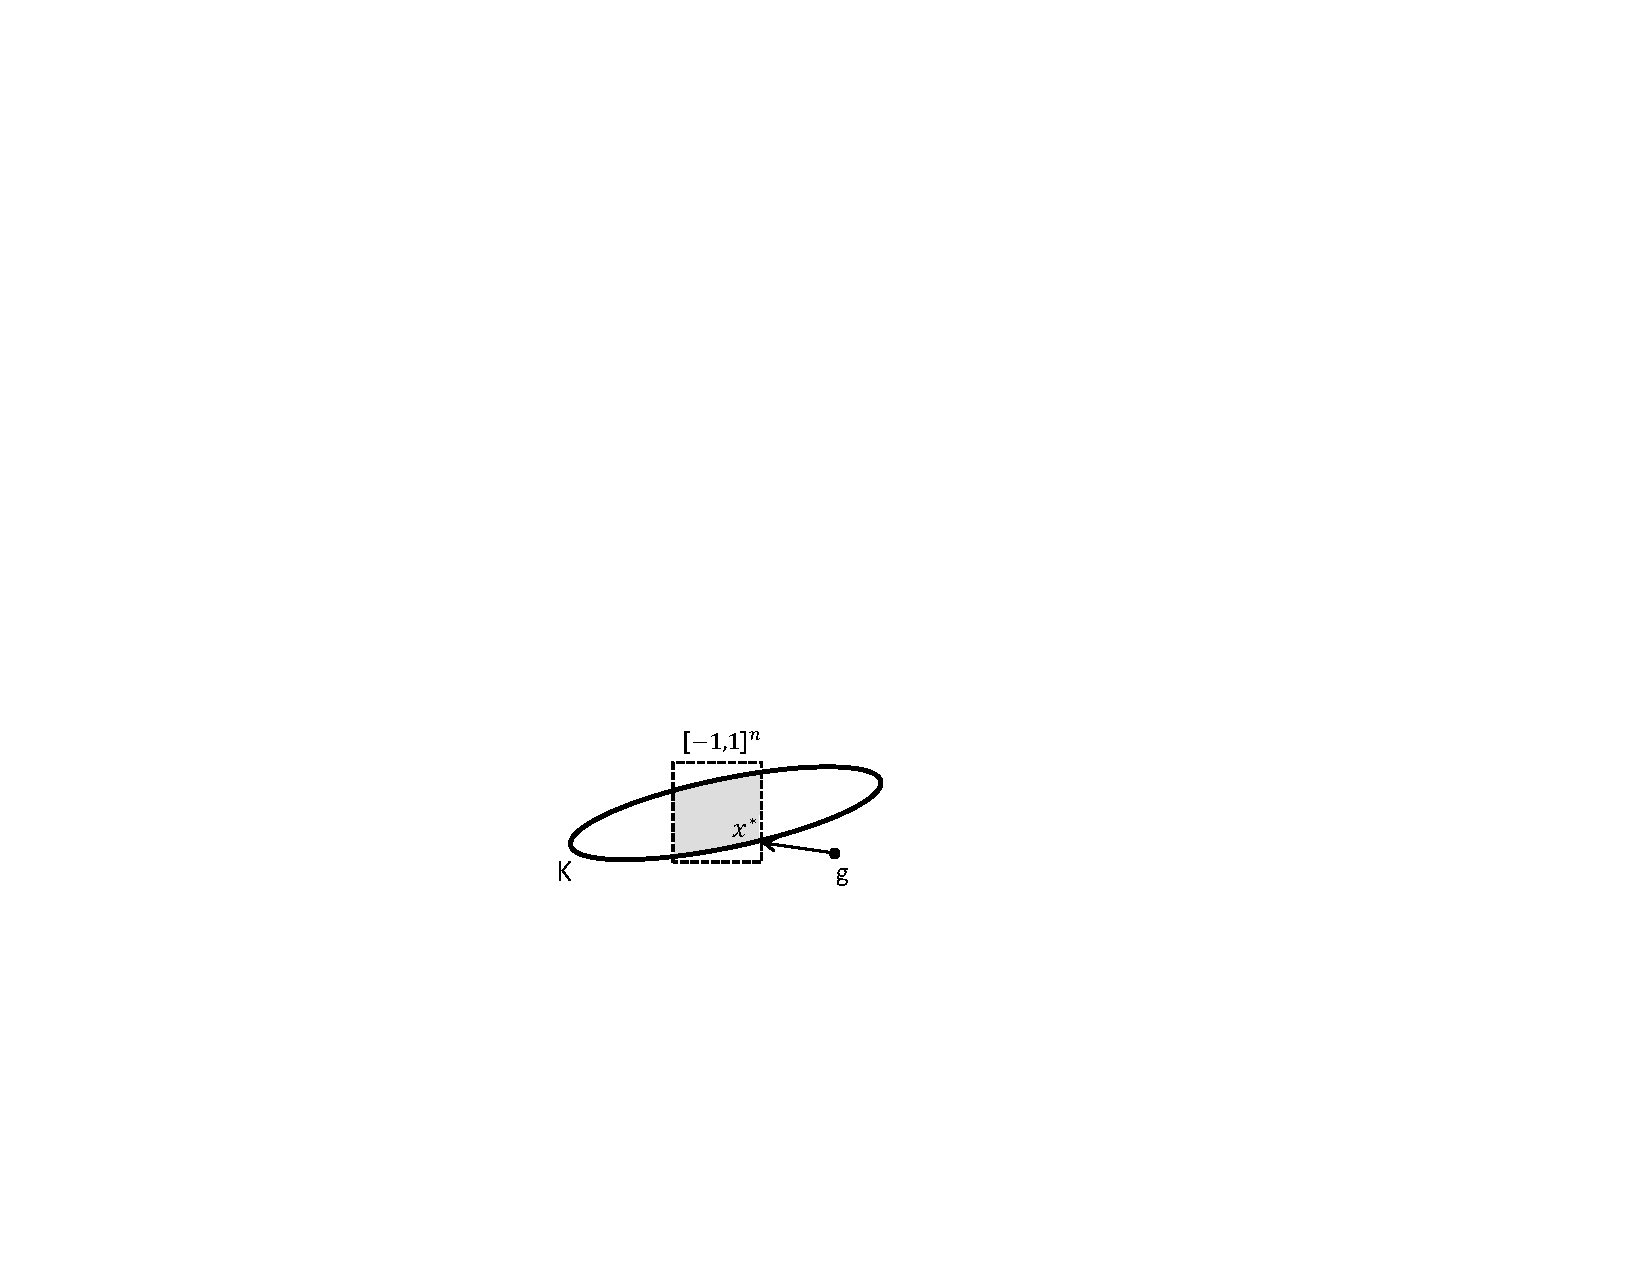
\includegraphics[scale=0.88, trim= {0mm 0mm 0mm 5mm}]{ch4-figures/figure-rothvoss.pdf}
    \caption{Rothvoss' Algorithm. The shaded area indicates $K\cap [-1,1]^n$, and $x^*$ is the closest point in $K\cap [-1,1]^n$ to the random Gaussian $g$.}
    \label{fig:ch4-rothvoss}
\end{figure}


Notice that $x^*$ can be determined efficiently, to any desired accuracy, by solving a convex program, as $f(x):=\|x-g\|_2$ is a convex function for any fixed $g$, and $K \cap [-1,1]^n$ is a convex set.
%In particular, using standard convex programming techniques, $x^*$ can be determined efficiently up to any arbitrary accuracy, given a 
All one needs is a membership oracle for $K$.
In fact, the objective function is strictly convex\footnote{i.e.,~$f(\lambda x + (1-\lambda) y) < \lambda f(x) + (1-\lambda) f(y)$ whenever $x\neq y$, $\lambda \in (0,1)$. Indeed, we can equivalently consider the objective $\|x-g\|^2_2$ and here, $\|\lambda x + (1-\lambda) y-g\|_2^2 - \lambda \|x-g\|_2^2 - (1-\lambda) \|y-g\|_2^2 = -\lambda(1-\lambda) \|x-y\|_2^2$ for all $g$.} and thus the optimum $x^*$ is always unique. 

\subsection{Analysis}
We now show that the algorithm satisfies Theorem \ref{thm:rothvoss-convex-discrepancy}. The analysis is very elegant, and uses two key observations about how 
the objective value $v^*:=\|x^*-g\|_2$ of the program \eqref{eq:rothvoss-algorithm} behaves. Note that both $x^*$
and $v^*$ are functions of $g$.
\medskip 

(i) With high probability, $v^* \geq c\sqrt{n}$, where $c>0$ is a universal constant independent of $\epsilon$. 

\medskip
(ii) If $x^*$ has fewer than $\delta n$ coordinates $x^*(i) \in \{-1,1\}$, then with high probability, $v^*$ must be small, roughly $O(\sqrt{(\epsilon + \delta \ln 1/\delta) n})$. 

%\smallskip

\medskip 
\noindent The result then follows directly from these observations.


\medskip

In light of this, let us take a brief detour to understand how the distance
$d(g,A):= \min\{\|x-g\|_2: x\in A\}$
of a point $g$ to a set $A \subset \R^n$ behaves, when $g \sim N(0,I_n)$ is chosen randomly. 

\medskip 
\noindent {\bf Fattenings and Gaussian Isoperimetric Inequality.}
 For $\delta>0$, let $A_\delta = \{x:d(x,A)\leq \delta\}$, the $\delta$-fattening of $A$, denote the set consisting of points within distance $\delta$ from $A$.
 Clearly, for any $g$,
 as $d(g,A) \leq \delta$ if and only if $g \in A_\delta$, we have that, for a standard Gaussian $g$ in $\R^n$,  \[\Pr[d(g,A) \leq \delta] = \gamma^n(A_\delta).\] 
 In other words, we can understand the distribution of the distance $d(g,A)$ by looking at the Gaussian measure of fattenings of $A$. 

 \smallskip
 The key tool to get a handle on $\gamma^n(A_\delta)$ is the classical Gaussian isoperimetric (GI) inequality~\cite{Borell75}, which states that among all sets with equal Gaussian measure, fattenings increase the measure of halfspaces the least. This is a Gaussian analog of the more classical isoperimetric inequality for volume (Lebesgue measure), which states that among all sets of equal volume, the Euclidean sphere has the smallest surface area. While the classical isoperimetric inequality is easily derived from the Brunn-Minkowski inequality \eqref{eq:ch3-bw}, the Gaussian isoperimetric inequality is a deeper fact. 
  
Formally, a halfspace is a set of the form $H:= \{x \in \R^n: \ip{u,x} \leq t\}$ for some unit vector $u \in \R^n$, and scalar $t\in \R$. The $\delta$-fattening of $H$ is $H_\delta:= \{x \in \R^n: \ip{u,x} \leq t+\delta\}$. By the rotational symmetry of Gaussians, we may assume that $u=e_1$ and thus,  
\[\gamma^n(H) = \Phi(t) = \gamma^1((-\infty,t]) = \int_{-\infty}^t (2\pi)^{-1/2} \exp(-t^2/2) \,dt.\] 

\begin{theorem}[GI Inequality]
\label{thm:gii}
    Let $A \subset \R^n$ be any measurable set and $H$ be any halfspace so that $\gamma^n(A) = \gamma^n(H)$. Then for every $\delta>0$, we have that  $\gamma^n(A_\delta) \geq  \gamma^n(H_\delta)$.
Equivalently,
for a set $A$, define the Gaussian isoperimetric function $t(A) := \Phi^{-1}(\gamma^n(A))$. 
Then, \[t(A_\delta) \geq t(H_\delta) = t(H)+\delta = t(A) + \delta.\]
\end{theorem}
This gives the following key fact --- if $\gamma^n(A)$ is not too small, then the measure concentrates close to $A$.
More quantitatively,

%far from the cube $[-1,1]^n$.
\begin{lemma} %Let $$.
%We have the following estimates for distance of $g$.
 %  \begin{enumerate} 
 \label{lm:ch4:measure-conc}
 Let $A\subset \R^n$ be a set with $\gamma^n(A) = \exp(-\beta n) \leq 1/2$. Then,
   $\Pr_{g\sim N(0,I_n)}[d(g,A) \geq  (8\beta n)^{1/2} ] < \exp(-\beta n)$.
\end{lemma}  
Let us first recall that $\Phi(0)=1/2$, and that  $\Phi(t) \leq \exp(-t^2/2)$ for $t \leq 0$, and by symmetry,  $\Phi(t) \geq 1- \exp(-t^2/2)$ for $t \geq 0$.

   \begin{proof}
Let $\delta := (8\beta n)^{1/2}$. 
We will show that $\gamma^n(A_\delta) \geq 1- \exp(-\beta n)$.
We use the notation in Theorem \ref{thm:gii}.

As $\Phi(t(A)) =\gamma^n(A) =\exp(-\beta n)\leq 1/2$, we have $t(A) \leq 0$ (as $\Phi(0)=1/2$). Using $\Phi(t) \leq \exp(-t^2/2)$ for $t \leq 0$, this gives $\exp(-\beta n) \leq \exp(-t(A)^2/2)$, and hence $t(A) \geq -(2\beta n)^{1/2}$.

By Theorem \ref{thm:gii}, $t(A_\delta) \geq -(2\beta n)^{1/2} + \delta = (2\beta n)^{1/2}$, and as $\Phi(t) \geq 1-\exp(-t^2/2)$ for $t>0$, this gives 
$\gamma^n(A_\delta) \geq 1- \exp(-\beta n)$.
\end{proof}

We now get back to proving Theorem \ref{thm:rothvoss-convex-discrepancy}.
%Let $K_{[n]}$ denote the body $K \cap [-1,1]^n$ (the reason for this notation will be clear soon)
We first show that the objective value $v^*=\|x^*-g\|_2$ in $\eqref{eq:rothvoss-algorithm}$ is typically quite large. 
 \begin{lemma}
 \label{lm:ch4:large-value}
        $\Pr_{g \sim N(0,I_n)}[v^* \leq  \sqrt{n}/6 ] = \exp(-\Omega(n))$.
        
        %In particular for $x^*$ defined in \eqref{}, 
        %\[\Pr[\|x^*-g\|_2 \geq \sqrt{n}/3] = 1- \exp(-%\Omega(n)).\] 
    \end{lemma}
 %  \end{enumerate}
\begin{proof}
As the domain $K \cap [-1,1]^n$ of $x$ in \eqref{eq:rothvoss-algorithm} is contained in  $[-1,1]^n$, it suffices to show that $\Pr[d(g,[-1,1]^n) \leq \sqrt{n}/6] = \exp(-\Omega(n))$.

Consider the squared  distance $d^2(g,[-1,1]^n) $.
%$= \sum_{i=1}^n  (\max(|g(i)|-1),0))^2$. 
Then each coordinate $i$ with $|g(i)|\geq 2$ contributes at least $1$, and this happens independently with probability $2 \gamma^1([2,\infty)) \geq 1/25$ for each $i$. Thus by standard Chernoff bounds $\Pr[d^2(g,[-1,1]^n) < n/36] = \exp(-\Omega(n))$.
\end{proof}

 \paragraph{Lower bound on the number of $\pm 1$ coordinates in $x^*$.}
To get a handle on when $x^*$ has few $\pm 1$ coordinates, we need a basic observation about convex programs.

%(proved below) ---
%If an optimum solution $x^*$ to a convex program does not satisfy some constraints with equality, then it remains optimum for the program obtained by dropping these constraints.

For a subset of coordinates $I \subseteq [n]$,
define the set $S(I):= %\cap_{i\in I} S(i) =
[-1,1]^I \times \R^{[n]\setminus I}$. In particular, $S([n])=[-1,1]^n$.  We have the following.
\begin{lemma}
\label{lm:ch4-rothvoss-convex}
    Fix some $g \in \R^n$. Let $x_g^*$ be the (unique) solution to \eqref{eq:rothvoss-algorithm},\footnote{We put the subscript $g$ to emphasize the dependence on $g$.} and let $I_g = \{i \in [n]: x_g^*(i) \in \{-1,1\}\}$ be the set of coordinates for which the constraints $x(i) \in [-1,1]$ are tight at $x_g^*$. Then \[\arg\min\{ \|x-g\|_2: x \in K \cap S(I_g)\} = x_g^*.\]

In other words, the optimizer to the convex program \eqref{eq:rothvoss-algorithm}  does not change upon dropping the constraints $x(i) \in [-1,1]$ for $i \notin I_g$.
\end{lemma}


\begin{proof}
Let us denote \[y_g^*=\arg\min\{ \|x-g\|_2: x \in K \cap S(I_g)\},\] and
suppose for the sake of contradiction that $y_g^*\neq x_g^*$.
Then, it must be that  $\|y_g^*-g\|_2 < \|x_g^*-g\|$, by strong convexity and as there are fewer constraints on $y_g^*$ (as $[-1,1]^n \subset  S(I_g^*)$).
Also, clearly, 
$y_g^*(i),x_g^*(i)  \in [-1,1]$ for each $i\in I_g^*$ (as these coordinate constraints are enforced). 

Next, crucially, by the definition of $I_g^*$ we have that $x_g^*(i) \in (0,1)$ for $i\notin I_g^*$.
So even though $y_g^*(i)$ may not lie in $[-1,1]$ for $i \notin I_g^*$, there exists some $\lambda \in (0,1)$ such that the point \[\tilde{x} = \lambda x_g^* + (1-\lambda) y_g^*\] lies in $[-1,1]^n$. As both $x_g^*,y_g^* \in K$ and $K$ is convex, we also have that $\tilde{x} \in K \cap [-1,1]^n$. This implies that $\tilde{x}$ is also a feasible solution to \eqref{eq:rothvoss-algorithm}. However, by strong convexity, \[\|\tilde{x}-g\|^2_2 < \lambda \|x_g^*-g\|_2^2 + (1-\lambda) \|y_g^*-g\|_2^2 <  \|x_g^*-g\|^2_2,\] which contradicts the optimality of $x_g^*$.
\end{proof}

For a subset of coordinates $I \subset [n]$, consider the objective value  
\[  v_g^*(I) := \text{min}\{ \|x-g\|_2: x \in K \cap S(I)\},\]
 in \eqref{eq:rothvoss-algorithm} when the constraints $x(i) \in [-1,1]$ are enforced only for $i\in I$. 
 
Clearly, the objective to \eqref{eq:rothvoss-algorithm} satisfies  $v^*_g =  v^*_g([n])\geq v^*_g(I)$ for all $I \subset [n]$ (as the domain $K \cap [-1,1]^n \subset K\cap S(I) $). 
On the other hand, 
Lemma \ref{lm:ch4-rothvoss-convex} gives that  \begin{equation}
    \label{eq:ch-rothvoss-val-relation}
    v^*_g = v^*_g(I_g) \text{ for every $g \in \R^n$}.
\end{equation}


\paragraph{Completing the proof.}
We now show that, with high probability over the choice of $g$, the value $v^*_g(I)$ is small for {\em every} $I$ such that $|I| \leq \delta n$.
By Lemma \ref{lm:ch4:large-value} and \eqref{eq:ch-rothvoss-val-relation}, this would imply that $|I_g|> \delta n $ with high probability, giving Theorem \ref{thm:rothvoss-convex-discrepancy}.
\begin{lemma}
For any fixed subset $I \subset [n]$ with $|I|\leq \delta n$, 
    \[\Pr_g[ v_g^*(I) \geq \sqrt{8(\epsilon+\delta) n}] \leq \exp(-(\epsilon+ \delta) n)   .\] 
\end{lemma}
\begin{proof}
As $v_g^*(I) = d(g,K\cap S(I))$, we apply Lemma \ref{lm:ch4:measure-conc} with $A= K \cap S(I)$.
To bound  $\gamma^n(A)$ from below, note that  $S(I) = \cap_{i\in I} S_i$ is an intersection of strips $S_i = \{x: |x(i)|\leq 1\}$,  and thus by the Sidak's Lemma \ref{lm:ch3-sidak}, 
   \[\gamma^n(K \cap S(I))  \geq \exp(-\epsilon n) \cdot (\gamma^1([-1,1]))^{|I|} \geq \exp(-(\epsilon+ \delta) n),\]
   where we use that $\gamma^1([-1,1]) \geq 0.682 \geq 1/e$ and $|I|\leq \delta n$. 
\end{proof}
Recall that, by standard estimates (e.g., Proposition 3.3.3 in~\cite{guruswami2012essential}), there are at most $2^{H(\delta)n}$ subsets $I \subset [n]$ with $|I|\leq \delta n$, where $H(\delta) = -\delta \log_2 \delta - (1-\delta)\log_2(1-\delta)$ is the binary entropy function. Applying a union bound over all such subsets, we have that,  with probability at least  $1- 2^{H(\delta) n} \exp(-(\epsilon+\delta)n)$, 
 \[  v^*_g(I) \leq \sqrt{8 (\epsilon + \delta)n} \,\,\,\, \text{ for all $I$ with }  |I|\leq \delta n.\]
%Choosing $\delta \leq c \eps/ \ln (1/\eps)$ for sufficiently small $c$, this probability is exponentially close to $1$, for any fixed $\epsilon$.
%
By \eqref{eq:ch-rothvoss-val-relation} this means that 
\[
\Pr[v_g^* \le \sqrt{8 (\epsilon + \delta)n}]
\ge 
1-2^{H(\delta) n} \exp(-(\epsilon + \delta)n)
- \Pr[|I_g| \ge \delta n].
\]
Choosing $\epsilon$ to be a sufficiently small constant, and $\delta \leq c \eps/ \ln (1/\eps)$ for sufficiently small $c$, and using Lemma \ref{lm:ch4:large-value}, we have that $|I_g| \ge \delta n$ with probability exponentially close to $1$. This completes the proof of Theorem \ref{thm:rothvoss-convex-discrepancy}. 

\section{Vector Discrepancy and SDPs}
\label{sec:vec-herdisc}
The partial coloring method can often give close to tight bounds for various general classes of matrices. E.g. any matrix $\mat$ with $m=n$ rows and entries in $[-1,1]$ has $O(\sqrt{n})$ discrepancy.
However, one can ask a stronger question ---
given {\em any} specific matrix $\mat$, can we efficiently find a coloring with discrepancy close to $\disc(\mat)$?

\smallskip 

Unfortunately, this is too much to hope for and discrepancy is very hard to approximate in general. For example, we will prove the following result in Chapter \ref{ch:bana-intro}.
\begin{theorem}
  For a set system $(\SS, [n])$ with $|\SS| = O(n)$ sets, it is $\mathsf{NP}$-hard to distinguish whether  $\disc(\SS) = 0$ or  $\disc(\SS) = \Omega(\sqrt{n})$.
\end{theorem}

This hardness result also suggests that LP or SDP based convex programming relaxations for discrepancy are unlikely to give useful information about the actual discrepancy $\disc(\mat)$.

While this is true in a sense, it turns out that SDPs can be very useful. In fact, the first algorithmic results for partial colorings were based on SDPs and random walks. In general, SDPs gives a flexible and powerful way to ``design'' random walks. Let us begin by exploring relaxations for discrepancy more closely. 

\medskip

\noindent {\bf LP relaxation.}
Recall that a linear program (LP) consists of variables $x(1),\ldots,x(n) \in \R$, viewed as a vector $x = (x(1),\ldots,x(n)) \in \R^n$, and the goal is to optimize some linear objective subject to some linear constraints. LPs can be solved optimally in polynomial time.
%in $n,m$, and the bit length of the input.

Given an $m\times n$ matrix $\mat$ with rows $v_1, \ldots, v_m \in \R^n$, the following is a natural LP relaxation for discrepancy,
\[ \min t \,\,\,\,  \text{ s.t. } \,\,    -t\leq  \ip{v_i ,x} \leq t,  \,\,\, \forall i \in [m]   \,\,\, \text{ and } \, -1 \leq x(j) \leq 1, \,\,\,\forall  j \in [n].\]
% \begin{align*}
%     & \min t  \\
% \text{s.t.}\quad  &    -t\leq  \ip{a_i, x} \leq t,  \quad \forall i \in [m] \\
% &  \quad  -1 \leq x_j \leq 1,  \quad \forall  j \in [n] 
% \end{align*} 
However this LP always has the trivial solution $x=\mathbf{0}$ with objective $t=0$, and hence is not at all useful.


% It is also the only approach we know for some problems such as the algorithmic version of Theorem \ref{th:rnd}, that we describe below in Theorem \ref{thm:pseduo-alg}. More importantly, it is quite flexible and can be extended in various ways by adding new SDP constraints, as we shall see later in Section \ref{sec:bana-alg}.
%when we consider Banaszczyk's approach.


%In hindsight, this seems natural as the statement of the partial coloring lemma can be viewed as a combination of iterated rounding and random coloring, as discussed below Theorem \ref{}.
\paragraph{Semidefinite Programs (SDPs).} 
These 
are a more general class of optimization problems, and an SDP can be viewed as an LP with
variables of the form $X(i,j)$ for $1 \leq i,j \leq n$, arranged as entries of an $n\times n$ matrix $X$, where we require that $X$ be symmetric and positive semidefinite (PSD), denoted  by $X \succeq 0$.

Formally, for matrices $A,B$, let $\ip{A, B} = \text{Tr}(A^TB) = \sum_{ij} A(i,j) B(i,j)$ denote the usual trace inner product for matrices. A SDP has the form
% There are $m$ arbitrary linear constraints on $x_{ij}$ of the type $\sum_{ij} a^k_{ij} x_{ij} \leq b^k$ for $k=1,\ldots,m$ and there is some linear objective function $\sum c_{ij} x_{ij}$. Moreover, we require the symmetry condition $x_{ij}=x_{ji}$.
% Finally, one imposes  That is, all its eigenvalues must be non-negative (this is well defined as $X$ is symmetric and hence has only real eigenvalues), and we denote this by $X \succeq 0$. To summarize, a general SDP has the following form.
\[
\max \ip{C,X}   \quad \text{s.t.} \quad  \ip{A_k, X}  \leq  b_k, \quad 1 \leq k \leq m,
\quad X  \succeq  0  \]
where $C,A_1,\ldots,A_m \in \R^{n\times n}$ are arbitrary, and it can be solved in polynomial time to any desired accuracy under mild assumptions. 

Recall that a matrix $X \succeq 0$ is PSD if and only if it is the Gram matrix of some vectors $w_1,\ldots,w_n \in \mathbb{R}^n$, i.e.,~$X(i,j)= \langle w_i,w_j \rangle$. So we can equivalently view SDPs as vector programs --- where the variables are the vectors $w_i$ and we can impose arbitrary linear constraints on their inner products (but not on the $w_i$ themselves).

\medskip

\noindent {\bf SDP relaxation for discrepancy.} 
Given a matrix $\mat \in \R^{m\times n}$, and some target discrepancy bound $\lambda$, consider the following SDP, where the colors $x(j)\in \pm 1$ are allowed to be arbitrary unit vectors, and the analogous quantity for the discrepancy $|\sum_j \mat(i,j) x(j)|$ of row $i$ becomes $\|\sum_j \mat(i,j) w_j\|_2$. See Figure \ref{fig:ch4-sdp} for an example.
%discrepancy $\lambda$. 
\begin{equation}
\label{eq:disc-sdp}
  \left\|\sum_{j} \mat(i,j) w_j\right\|_2^2 \leq\lambda^2 \quad \text{for } i \in [m],  \qquad \|w_j\|_2^2  =  1  \quad {j\in [n].}
\end{equation}
\begin{figure}[hbtp!]
    \centering
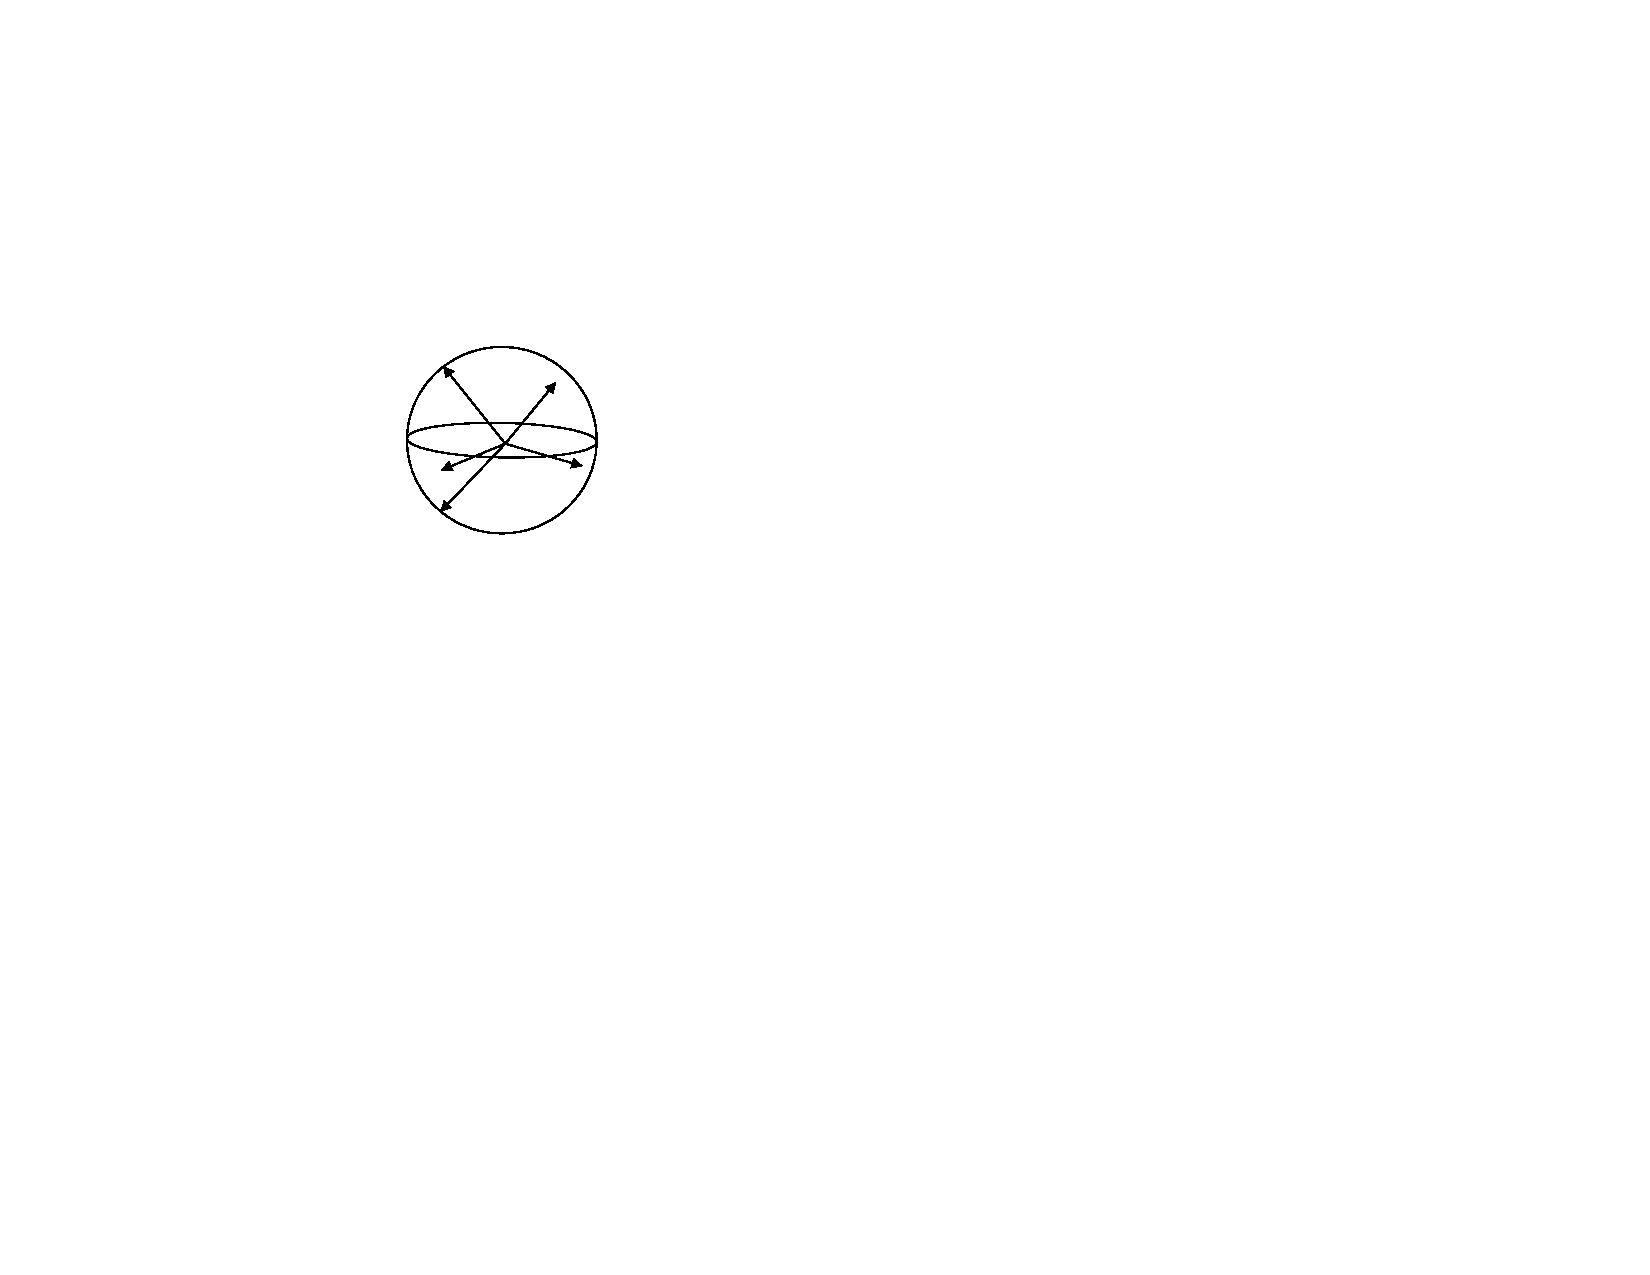
\includegraphics[scale=0.88, trim= {0mm 0mm 0mm 5mm}]{ch4-figures/figures-ch4-sdp.pdf}
    \caption{The unit vectors $w_j \in \R^n$ in the SDP solution.}
    \label{fig:ch4-sdp}
\end{figure}


Let us define the vector discrepancy of matrix as follows.
\begin{definition} We define
the vector discrepancy 
    $\vdisc(\mat)$ of a matrix $\mat$ as the smallest $\lambda\geq 0$ for which \eqref{eq:disc-sdp} is feasible.
\end{definition}
Clearly \ref{eq:disc-sdp} implies $\vdisc(\mat) \leq \disc(\mat)$.
%as for any coloring $x \in \{-1,1\}^n$, setting $w_j= x(j) e_1$ has the same discrepancy.
% Notice that \eqref{} can be written equivalently as, $\ip{A_i,X} \leq \lambda^2$ for $i\in [m]$ where $A_i= a_ia_i^T$,   $X_{jj}=1$ for $j\in [n]$ and $X \succ 0$.
However, at first glance, vector colorings do not seem to give useful information. E.g.,~for any matrix $\mat$ with entries in $[-1,1]$ (as in Spencer's theorem~\ref{thm:ch3-spencer}), the solution $w_i=e_i$, the $i$-th standard basis vector, is always feasible with $\lambda = n^{1/2}$.
%So this does not seem to give any useful information.
%to beat the random coloring bound.

Interestingly however, this SDP becomes quite useful when $\lambda \ll n^{1/2}$, as it gives non-trivial correlations between the vectors $w_i$ that we can exploit. In particular, even though $\disc(\mat)$ is hard to approximate (as we will prove in Chapter~\ref{ch:gamma2}), we can show the following instance-wise result.

\begin{theorem}
\label{thm:pseduo-alg}
Given any $m\times n$ matrix $\mat$, one can find a coloring with discrepancy $O((\log m \log n)^{1/2} \herdisc(\mat))$ in polynomial time.
\end{theorem}
We first describe the algorithm and then prove Theorem \ref{thm:pseduo-alg}.
\subsection{Algorithm}
At a high level, the algorithm performs a random walk as in the Lovett-Meka algorithm. However, instead of taking a random step in a subspace, the random increments for coordinates are carefully correlated so that the discrepancy increment for each row of $\mat$ is small. In particular, at each step it solves the SDP in \eqref{eq:disc-sdp}  (restricted to coordinates with colors not yet $\pm 1$) with $\lambda = \herdisc(\mat)$, and generates a step of the walk by using this solution as the covariance matrix.  
We now describe this formally.


%$v_i$ to any vector $g \in \R^n$ nicely maintains the correlations as the resulting $y_j= \langle g,v_j \rangle$ also satisfy
%\[\sum_{j} \mat(i,j) y_j  =\langle  g, \sum_{j} \mat(i,j) v_{j}\rangle =  \langle g,\mathbf{0}\rangle =0.\]
%\leq \|g\|_2  \cdot \|\sum_{i\in S_j} v_i\|_2,$$
%implying that $\sum_{i \in S_j} y_i$ is also small if $\|\sum_{i\in %S_j} v_i\|$ is small.

%with high probability (for some large enough constant $c$).
%Moreover, for any $j$, the discrepancy $|\sum_{i \in S_j} y_i | = O(\lambda (\log n)^{1/2})$ with high probability.
%Perhaps, one could now hope to round these $y_i$'s to $\pm 1$ without increasing the discrepancy substantially.
%as is done in other contexts such as cut-norm minimization \cite{}, correlation clustering \cite{cut-norm,groethendieck}.



\paragraph{ Algorithm.} Fix a small step size $\gamma = \max_{i,j}|\mat(i,j)|/n^2$  and let $\delta = 4 \gamma \log(2mn/\gamma)$. 
Let $\lambda = \herdisc(\mat)$.\footnote{While we do not know $\herdisc(\mat)$, we can do a binary search on $\lambda$.}  

Let $x_{t-1}$ denote the coloring and let $F_t = \{j: |x_{t-1}(j)| > 1-\delta\}$ be the set of fixed elements at the end of time step $t-1$. 
Initialize $x_0(j) =0$ for $j\in [n]$ and $F_1= \emptyset$. 

\medskip 

 \noindent At each time $t=1,2,\ldots,\ell = (4 \log n)/\gamma^2$, do the following. 
 
\smallskip 

(i)  Solve the SDP
%\item Let $(p,q)$ denote the current phase at time $t$.
 \begin{align*}
     & \|\sum_{j} \mat(i,j) w^t_j\|_2^2  \leq   \lambda^2 \quad \forall i\in [m],\\
     &  \|w^t_j\|_2^2  =   1   \text{ if }  j \not\in F_t,\text{ and }
   \| w^t_j\|_2^2 =  0 \text{ otherwise}. 
 \end{align*}
 
%This SDP is feasible as setting $v_i \cdot v_j =\mathcal{X}(i) \mathcal{X}(j)$, where $\mathcal{X}$ is the minimum discrepancy coloring of the set system restricted to $\mat(t-1)$ is a valid solution
%Construct $u^{t}= \in \mathbb{R}^n$ as follows:

(ii) Sample $g_t \sim N(0,I_n)$, and set 
%obtained by choosing each coordinate $g(i)$ independently from the distribution $\mathcal{N}(0,1)$. For each $i \in [n]$
\[x_t(j) = x_{t-1}(j) + \gamma \langle g_t,w^t_j \rangle \text{ for each $j\in [n]$}.\]
\,\,\,\,\,\,\,\,\, Set $F_{t+1} = \{j: |x_t(j)| > 1-\delta\}$.
% \item
% \label{freeze}
% Set $F^t=F^{t-1}$. For each $i$, freeze $i$ if , and update $F^{t}=F^{t} \cup \{i\}$.
  %F^{t}= if $x_t(i)\geq 1-1/n$ or  set $x_t(i)=-1$ if $x_t(i) < -1+1/n$.\\
%Update $A(t)$ accordingly.
%\end{enumerate}
%\item After time $t=\ell$, 

\medskip 
\noindent Output the final coloring $x(j)=\text{sign}(x_{\ell}(j))$.


\subsection{Analysis}
The ideas are similar to those in Section \ref{sec:lm}.

First, note that the SDP is always feasible at each time $t$. This is because we set $\lambda = \herdisc(\mat)$, and hence  $\disc(\mat(*,[n]\setminus F_t)) \le \lambda.$ 

Let us now consider how the colorings $x_t$ and the row discrepancies evolve.
%We now sketch the proof of Theorem \ref{}.
%that this algorithm produces a coloring with discrepancy $O((\log m\log n)^{1/2} \herdisc(\mat))$ with
%high probability.
%The proof relies on two simple ideas, that we first describe informally.
%\vspace{5mm}
%\noindent \paragraph{ The proof sketch:}
%First we show that all elements are frozen by time $\ell$ with high probability.
Fix some element $j$. Its color $x_t(j)$ starts at $0$ and evolves as a martingale with updates 
\(\Delta x_t(j)= \gamma \langle w^t_j,g_t\rangle,\) % \sim N(0,\gamma^2 \|w^t_j\|^2).\]
which are distributed as a Gaussian with mean $0$ and variance $\gamma^2 \|w^t_j\|^2$.
Similarly, for the $i$-th row $v_i$ of $\mat$, its discrepancy $x_t(v_i) := \sum_{j} \mat(i,j) x_t(j)$ is $0$ at $t=0$, and evolves as a martingale with increments \[\sum_j \mat(i,j) \Delta x_t(j)  = \sum_{j} \gamma \langle g_t,\sum_j \mat(i,j) w^t_j \rangle,\]
% \sim N\left((0,\gamma^2 \left\|\sum_j \mat(i,j) w^t_j\right\|^2\right).\]
where the right hand side is a Gaussian with mean $0$ and variance equal to \(\gamma^2 \left\|\sum_j \mat(i,j) w^t_j\right\|^2.\)

\medskip
\noindent {\bf The discrepancy bound.}
 Fix some row $i$. As $\| \sum_j \mat(i,j) w^t_j\|^2 \leq \lambda^2$ by the SDP constraint, the discrepancy increment  $\Delta x_t(v_i)$ is a Gaussian with mean $0$ and variance bounded above by $\gamma^2 \lambda^2$. 
%This is distributed as $N(0, \gamma_^2$  \leq  \gamma^2 \lambda^2 $ by the SDP constraint.
%Thus (roughly speaking) $x^t(S_j)$ evolves as a random walk with steps $N(0,\leq \gamma \lambda)$.
%Thus, after $\ell$ steps, with constant probability, $x^{\ell}(S_j)$ would be no more than $ O(\sqrt{\ell} \gamma \lambda) = O(\sqrt{\log n} \lambda)$.
So 
by Lemma \ref{ch4:lm-martingale-bound}, 
\[
\Pr [ |x_\ell(v_i)| \geq \ell^{1/2}  \gamma \lambda \cdot c (\log m)^{1/2}] \leq  2\exp(-(c^2 \log m)/2).\]
Plugging $\ell = (4 \log n)/\gamma^2$ and choosing $c$ large enough, a union bound over the $m$ rows gives that $\disc(\mat,\col) = O(\lambda\, (\log m \log n)^{1/2})$ whp.
%at most $\exp(-2 \log m) = 1/n^2$, and the result follows by a union bound over the $m$ rows.


\medskip
\noindent {\bf All elements become fixed.}
As long as $j \not \in F_t$ is alive, the SDP constraint ensures that 
%|x_\ell(j) \geq 1$ for all $j$. 
$\|w^t_j\|_2=1$. So, $\Delta x_t(j)$ is a mean $0$ Gaussian with variance $\gamma^2$, and at each step,
%Strictly speaking, this is not true as the previous choices of $g^{t'}$ determine whether $i$ is frozen by time $t$ or not, and hence determine whether $u^t(i)=0$ or not (but let us ignore this point here).
%More precisely, $x^t(i)$ forms martingale with $N(0,\gamma^2)$
% increments, until it is absorbed at $\pm 1$.} of all previous increments $u^{t'}(i)$, where $t'<t$.
$x_{t}^2(j)$ increases  on average by \[\E[x_{t}^2(j)|x_{t-1}(j)] - x^2_{t-1}(j)  = \E[(\Delta x_t(j))^2|x_{t-1}] =\gamma^2.\] 
A similar argument as in Lemma \ref{lem:lm-vl} gives that $x_t(j)$ will reach $\pm 1-\delta$ in
$(2/\gamma^2)$ steps with probability at least $1/2$ (irrespective of where it started).
Dividing $\ell = 4\log n/\gamma^2$ into $2 \log n$ intervals of size $2/\gamma^2$, the probability that $j$ stays active (i.e., is not fixed) till the end of the algorithm is at most $1/n^2$. The result then follows by a union bound over the $n$ elements.

\medskip
\noindent
{\bf Rounding Error.}
We condition on the event that at the end of the algorithm all elements are fixed, i.e., $F_{\ell+1} = [n]$.
As a color is not updated once $|x_t(j)|\geq 1-\delta$, our choice of $\delta$ ensures that  $|x_\ell(j)| \leq 1$ for all $j$ with high probability.
So, rounding the $x_\ell(j)$ to $\pm 1$ at the end incurs error at most $n \delta =  o(\max_{ij}|\mat(i,j)|)$ per row, which is negligible as $\herdisc(\mat) \geq \max_{ij} |\mat(i,j)|$.




\section{Bibliographic Notes}
\label{sec:ch4-notes}
The first algorithmic approach for partial coloring was given by Bansal \cite{B10}, who gave efficient algorithms for various applications such as the $O(n^{1/2})$ bound for Spencer's problem with $m=O(n)$ sets, and the $O(t^{1/2} \log n)$ bound for the Beck-Fiala problem. His approach was based on SDPs and random walks. Theorem \ref{thm:pseduo-alg} is also from \cite{B10}. 

Even though the approach of \cite{B10} gave efficient algorithms, the algorithms relied on the existence of partial coloring as given by Theorem \ref{lm:ch3-partial} to argue the feasibility of the underlying SDPs, and hence was not fully constructive.
The first truly constructive algorithm for the partial coloring method was given by Lovett and Meka \cite{lovettmeka}, which we described in Section \ref{sec:lm},  

The algorithm in Section \ref{sec:ch4-rothvoss}, for general convex bodies, is due to Rothvoss \cite{Rothvoss17}.
Another elegant algorithm, that also works for general symmetric convex bodies $K$, is due to Eldan and Singh \cite{EldanS18}. This algorithm is also very simple to state ----- Pick a uniformly random direction $\theta \in \R^n$ and solve the linear program $\max \ip{\theta,x}$ subject to $x \in K \cap [-1,1]$. 

The Gaussian Isoperimetric inequality was proved by Sudakov and Tsirelson \cite{sudakov-tsirelson78} and independently by Borell \cite{Borell75}. Several other proofs are now known and we refer to the note by Ledoux \cite{Ledoux-survey}. We will see a generalization of this inequality called  Ehrhard's inequality in Chapter \ref{ch:bana-proof}.

Interestingly Rothvoss's algorithm enjoys a guarantee similar to Theorem~\ref{thm:pseduo-alg}. Dadush, Nikolov, Talwar, and Tomczak-Jaegermann showed that, using Rothvoss's algorithm with $K = \{\col \in \R^n: \|\mat \col\|_{\infty} \le C\herdisc(\mat)\}$ for a large enough constant $C$, we get a partial coloring with discrepancy $O(\herdisc(\mat))$. We can then extend the partial coloring to a full coloring $\col$ with discrepancy $O(\log(n)\herdisc(\mat))$~\cite{anynorm}. They also showed that this holds more generally for discrepancy measured in any norm. 


The SDP-based approach in Section \ref{sec:vec-herdisc} was also used in \cite{BDG16}, with some additional constraints, to obtain the first algorithmic bound for the Koml\'{o}s problem, matching Banaszczyk's non-constructive  bound \cite{Bana98}. We will see Banaszczyk's method in Chapter \ref{ch:bana-intro} and the algorithm of \cite{BDG16} in Chapter \ref{ch:algo-komlos-bana}.  



Several other algorithmic approaches have also been developed. 
These are typically stated for specific problems, but often the underlying idea is more generally applicable.
Harvey, Schwartz and Singh \cite{HSS14}  developed an algorithm based on inscribing ellipsoids and random walks.  
Rothvoss and Reis \cite{ReisR23} consider another variant that combines ideas from the algorithms in Section \ref{sec:lm} and \ref{sec:ch4-rothvoss}.
More recently, deterministic algorithms based on 
barrier potential functions \cite{BansalLV22} and regularized optimization \cite{PesentiV23} have also been developed. Remarkably, the approach of \cite{PesentiV23}, in addition to being algorithmic, also improves the constant for Spencer's problem for $m=n$ sets from  $5.32$ in \cite{spencer1985} to $3.67$.


Beyond discrepancy, these approaches have also led to several new results in areas such as approximation algorithms, computational geometry, machine learning, differential privacy and graph sparsification. We do not discuss these here due to lack of space, but would like to highlight the breakthrough result of Rothvoss \cite{Rothvoss16} and Hoberg and Rothvoss  \cite{HobergR19}, who used these ideas to obtain an additive $O(\log n)$ approximation for the classical bin packing problem, improving on the long-standing $O(\log^2 n)$ bound by Karmarkar and Karp \cite{KarmarkarK82}. For a general connection between discrepancy and rounding techniques, we refer to \cite{Bansal19}.

There has also been a lot of recent interest in designing discrepancy algorithms with fast running times \cite{JainSS23, JambulapatiRT24}. In Chapter \ref{ch:online}, we will see a beautiful algorithm due to Alweiss, Liu and Sawhney \cite{alweiss2020discrepancy}, that runs in time linear in $\text{nnz}(\mat)$, the number of non-zero entries of $\mat$, and also works in the online setting.

Matou\v{s}ek \cite{Matousek-detlb} used the connection between vector discrepancy and hereditary discrepancy in Section \ref{sec:vec-herdisc}, together with SDP duality, to show a remarkable result that the hereditary discrepancy of any matrix $\mat$ is tightly characterized by the so-called determinant lower bound (see Chapter \ref{ch:gamma2} for the definition). The lower bound  $\detlb(\mat) \leq \herdisc(\mat)$ was shown by Lov\'asz, Spencer and Vesztergombi~\cite{LSV}, and we give an exposition of their proof in Chapter~\ref{ch:gamma2}. Matou\v{s}ek showed the upper bound $\herdisc(\mat) \leq O(\log n)^{3/2} \detlb(\mat)$.
This was further improved by Jiang and Reis \cite{JiangReis22} to a logarithmic bound, which is also the best possible~\cite{LiNikolov24}.
We will explore some related ideas further in Chapter \ref{ch:gamma2}. 


% \section{Lovett Meka}
% Add exposition from the chapter I wrote for panorama of discrepancy. 
% That was not set systems. So need to fix notation etc.

% \section{Rothvoss proof}
% The Lovett-Meka algorithm crucially uses the face structure of the polytope and does not seem to generalize to general convex bodies in the sense of Theorem \ref{th:gluskin}. 
% In general, approximating a general convex body $K$ to a reasonable accuracy requires exponentially many facets. However, in that case the condition \eqref{eq:ent} becomes quite weak and does not give anything useful.

% We now describe an elegant result due to Rothvoss \cite{}, that gives an algorithmic version of the partial coloring result due to Gluskin and Giannopoulous for general convex bodies.

% \begin{theorem}
% \label{thm:rothvoss-convex-discrepancy}
%     Let $\epsilon, \delta>0$ be sufficiently small constants\footnote{The constants $\epsilon,\delta$ can be computed explicitly \cite{}, but we avoid this here for ease of exposition.}, and let $K \in \R^n$ be a symmetric convex body with Gaussian measure $\gamma_n(K) \geq \exp(-\epsilon n)$. Then there is a polynomial time algorithm that finds a point $x \in K \cap[-1,1]^n$ with $x_i\in \{-1,1\}$ for at least $\delta n$ coordinates.  
% \end{theorem}
% %In contrast to  the Lovett-Meka algorithm which moves inside the cube, the algorithm of Rothvoss is based on literally thinking outside the box, 
% Amazingly, the algorithm can be described in a single line!

%  \paragraph{Algorithm:}
%   Sample a random Gaussian $g \sim N(0,I_n)$, and output the point $x^*$ in $K \cap [-1,1]^n$ closest to $g$. That is, output
% \begin{equation}
%     \label{eq:rothvoss-algorithm}
% x^* = \text{argmin} \,\{ \|x-g\|_2 : x \in K \cap [-1,1]^n\}.
% \end{equation}
% Notice that $x^*$ can be determined efficiently, to any desired accuracy, by solving a simple convex program, as $\|x-g\|_2$ is a convex function and $K \cap [-1,1]^n$ is a convex set.
% %In particular, using standard convex programming techniques, $x^*$ can be determined efficiently up to any arbitrary accuracy, given a 
% All one needs is a membership oracle for $K$.

% To prove Theorem \ref{thm:rothvoss-convex-discrepancy}, we will show that
% %\begin{theorem}
% the point $x^*$  in \eqref{eq:rothvoss-algorithm} satisfies the guarantee of Theorem \ref{thm:rothvoss-convex-discrepancy} with high probability (whp).
% %\end{theorem}

% The idea of the proof will be to show that the cube $[-1,1]^n$ constrains the solution $x^*$ much more than $K$. This will cause 
% many cube constraints to be {\em tight} for $x^*$, leading to $\pm 1$ values in those coordinates. Intuitively, this is because $K$ has much larger measure than the cube, so a random Gaussian $g$ will have distance only $O(\sqrt{\eps n})$ from $K$, but its distance  from $[-1,1]^n$ will be $\Omega(\sqrt{n})$.  We now give the details.

% \paragraph{Distance estimates.}
%  For a set $A$, let $d(x,A):= \min\{\|x-y\|_2: y\in A\}$ denote the distance of $x$ to $A$. For $\delta>0$, let $K_\delta = \{x:d(x,A)\leq \delta)$ be the $\delta$-fattening of $K$, consisting of points at distance at most $\delta$ from $A$. 
% A halfspace is a set of the form $H:= \{x \in \R^n: \ip{v,x} \leq t\}$ for some unit vector $v \in \R^n$ and $t\in \R$.

% A key result on Gaussian measure of sets and their fattenings is the Gaussian isoperimetric inequality due to \cite{}. We refer to an elegant proof due to Bobkov \ref{}. 
% \begin{theorem}[Gaussian Isoperimetric Inequality]
%     Let $A \subset \R^n$ be a measurable set and $H$ be any halfspace so that $\gamma_n(A) = \gamma_n(H)$. Then  $\gamma_n(A_\delta) \geq \gamma_n(H_\delta)$ for any $\delta>0$. 
% \end{theorem}
% In other words, among all sets with the same measure, fattenings increase the measure of halfspaces by the least amount. Moreover, by the rotational symmetry of Gaussians, as any halfspace $H =\{x:\ip{v,x}  \leq t\}$ has Gaussian measure $\Phi(t) = \gamma_1((-\infty,t]) = \int_{-\infty}^t \frac{1}{\sqrt{2\pi}} \exp(-t^2/2)$, this often reduces volume estimates of bodies in $\R^n$ to the $1$-dimensional case.

% We recall the following basic estimates.
% For any $t \leq 0$, we have $\Phi(t) \leq \exp(-t^2/2)/2$. By  symmetry  this gives  $1-\Phi(t) \leq \exp(-t^2/2)/2$ for $t\geq 0$, and that $\gamma_1([-1,1])\geq e^{-1/2}$.

% We can now show that a random gaussian $g \sim N(0,I_n)$ is typically close to $K$, but the objective value $\|x^*-g\|$ in $\eqref{eq:rothvoss-algorithm}$ is much larger. 
% %far from the cube $[-1,1]^n$.
% \begin{lemma} Let $g \sim N(0,I_n)$.
% %We have the following estimates for distance of $g$.
%  %  \begin{enumerate} 
%    Then for any measurable set $A$ with $\gamma_n(A) = \exp(-\eps n) \leq 1/2$, we have  \[\Pr[d(g,A) \geq 3 \sqrt{\eps n} ] \leq \exp(-\eps n).\]
% \end{lemma}  
%    \begin{proof}
% Equivalently, we show that $\gamma_n\left(A_{3\sqrt{\eps n}}\right) \geq 1- \exp(-\eps n)$.
% Let $t <0$ so that the halfspace $H = \{x\in \R^n:x_1\leq t\}$ has measure $\gamma_n(H) = \gamma_n(A)$. Then, we claim that  $t > -3/2 \sqrt{\eps n}$ as,
% \[ \Phi(3/2 \sqrt{\eps n}) \leq \exp(- 9/8 \eps n)/2 \leq \exp(-\eps n).\]
% Thus by the Gaussian isoperimetric inequality, \[\gamma_n\left(A_{3 \sqrt{\eps n}} \right) \geq \gamma_n \left(H_{3\sqrt{\eps n}}\right) =\Phi(t + 3 \sqrt{\eps n}) \geq \Phi(3/2 \sqrt{\eps n}) \geq 1- \exp(-\eps n).\qedhere\] 
% \end{proof}

%     \begin{lemma}
%         Let $g \sim N(0,I_n)$. Then
%         $\Pr[ \|x^*-g\|_2 \geq  \sqrt{n}/3 ] = 1- \exp(-\Omega(n))$.
        
%         %In particular for $x^*$ defined in \eqref{}, 
%         %\[\Pr[\|x^*-g\|_2 \geq \sqrt{n}/3] = 1- \exp(-%\Omega(n)).\] 
%     \end{lemma}
%  %  \end{enumerate}
% \begin{proof}
% As the domain $K \cap [-1,1]^n$ of $x$ in \eqref{eq:rothvoss-algorithm} is contained in  $[-1,1]^n$, it suffices to show that $\Pr[d(g,[-1,1]^n) \geq \sqrt{n}/3] = 1- \exp(-\Omega(n))$.

% Now, for any point $y\in \R^n$, its squared distance  to the cube is exactly $(d(y,[-1,1]^n))^2=\sum_{i=1}^n  (\max(|y_i|-1),0))^2$. By the symmetry of Gaussians, it suffices to consider each coordinate of $g$ separately. 
% Then
% \[ \E[(d(g_1,[-1,1])^2] = 2\int_{1}^\infty (x-1)^2 \frac{1}{\sqrt{2\pi}} \exp(-x^2/2) dx \geq 0.1507 \geq 1/7.\]
% As the $g_i$ are independent for $i\in [n]$, the result follows by standard Chernoff bounds. 
% \end{proof}

%  \paragraph{Lower bounding the number of $\pm 1$ coordinates in $x^*$.}
% Given some $g$, let $x^*$ be some optimum solution to \eqref{}. Then as the function $f(x)=\|x-g\|_2^2$ is strictly convex (i.e.,~$f(\lambda x + (1-\lambda) y) < \lambda f(x) + (1-\lambda) f(y)$ whenever $x\neq y$ and $\lambda \in (0,1)$), $x^*$ must be the unique optimum. 

%  For $i\in [n]$, let $S(i)$ denote the strip $S(i)= \{x\in \R^n:x_i \in [-1,1]\}$, and for a subset of coordinates $I \subseteq [n]$, let $S(I)= \cap_{i\in I} S(i) = [-1,1]^I \times \R^{[n]\setminus I}$.
%  %Note that $S([n])$ is imply the cube $[-1,1]^n$.  

% %and let $B_I$ denote that event that $y^*(I) = x^*$.


% A simple but key observation is the following.
% \begin{lemma}
%     Given some $g \in \R^n$, let $x^*$ be the optimum solution to \eqref{eq:rothvoss-algorithm}, and let $I^* = \{i \in [n]: x_i^* \in \{-1,1\}\}$ be the set of coordinates where the constraints $x_i \in [-1,1]$ are tight for $x^*$. Let $y^* =\text{argmin}\{ \|x-g\|_2: x \in K \cap S(I^*)\}$. 
%     Then $y^*=x^*$. 
% \end{lemma}
% \begin{proof}
% %Let $y^*=\text{argmin}\{ \|x-g\|_2: y \in K \cap S(I)\}$ and 
% Suppose for the sake of contradiction that $y^*\neq x^*$.
% Then $\|y^*-g\|_2 < \|x^*-g\|$  as $[-1,1]^n \subset  S(I^*)$. As $y_i^*,x_i^* \in [-1,1]$ for $i\in I^*$ and $x_i^* \in (0,1)$ for $i\notin I^*$ (so $x^*$ has some slack to move in these directions), there must exist some $\lambda \in (0,1)$ such that $x = \lambda x^* + (1-\lambda) y^* \in [-1,1]^n$. As $x^*,y^* \in K$, we have $x \in K \cap [-1,1]^n$ and it is a feasible solution to \eqref{eq:rothvoss-algorithm}. But then by strong convexity, $\|x-g\|^2_2 < \lambda \|x^*-g\|_2^2 + (1-\lambda) \|y^*-g\|_2^2 <  \|x^*-g\|_2$, contradicting the choice of $x^*$.
% \end{proof}

% We can now finish the proof. 

% For $I \subset [n]$, let $y^*(I) = \text{argmin}\{ \|y-g\|_2: y \in K \cap S(I)\}$.
% By Sidak-Khatri Lemma \ref{},
% $\gamma_n(K \cap S(I))  \geq \gamma_n (K) \cdot \gamma_n (S(I)) = \gamma_n(K) \cdot \gamma_1([-1,1])^{|I|} \geq \exp(-\eps n - |I|/2).$.

% TODO: 
% \begin{enumerate}
% \item Add Lovett Meka. Have older notes for set system. Need to change notation and adapt.
%     \item Complete the Rothvoss proof
%     \item Add figures for both algorithms
%     \item Add Exercises
%\end{enumerate}